%--------------------------------------------------------------
% GLoBES Poster (A0, portrait)
%--------------------------------------------------------------
% Note: This LaTeX file requires the TikZ/PGF package, and
%       works only with pdflatex v1.30 or higher
%--------------------------------------------------------------
\documentclass[portrait,a0]{a0poster}

\usepackage{multicol}
\usepackage{calc}
\usepackage[sort&compress]{natbib}
\usepackage{amsmath}
\usepackage{fancybox}
\usepackage{graphicx,color,tikz}
\usepackage{shapepar}
\usepackage[english]{babel}

% Set up natbib package
\setlength{\bibsep}{0cm}
\bibpunct{[}{]}{,}{n}{}{,}

\setlength{\unitlength}{1cm}
\setlength{\fboxrule}{0.5mm}
\newcommand{\GeV}{\,\mathrm{GeV}}

% Quantum mechanical notation
\newcommand{\bra}[1]{\ensuremath{\langle #1 |}}   % Bra vector
\newcommand{\ket}[1]{\ensuremath{| #1 \rangle}}   % Ket vector
\newcommand{\amp}[3]{\ensuremath{\left\langle #1 \,\left|\, #2 \,\right|\, #3 \right\rangle}}  % QM amplitude
\newcommand{\sprod}[2]{\ensuremath{\left\langle #1 | #2 \right\rangle}}  % QM scalar product
\newcommand{\ev}[1]{\ensuremath{\left\langle #1 \right\rangle}} % Expectation value


% Color definitions
\definecolor{bgcolor}{rgb}{0.6, 0.0, 0.0}
\definecolor{boxcolor}{rgb}{0.95, 0.95, 0.85}
\definecolor{headingframe}{rgb}{1.0, 0.7, 0.0}
\definecolor{headingbg}{rgb}{1.0, 0.9, 0.6}
\definecolor{emphcolor}{rgb}{0.8, 0.0, 0.0}
\definecolor{dr}{rgb}{0.6, 0, 0}
\definecolor{dg}{rgb}{0, 0.6, 0}
\definecolor{db}{rgb}{0, 0, 0.6}
\definecolor{dy}{rgb}{0.6, 0.6, 0}
\newcommand{\emphcolor}[1]{\textcolor{emphcolor}{#1}}
\newcommand{\dr}[1]{\textcolor{dr}{#1}}
\newcommand{\dg}[1]{\textcolor{dg}{#1}}
\newcommand{\db}[1]{\textcolor{db}{#1}}
\newcommand{\dy}[1]{\textcolor{dy}{#1}}
\renewcommand{\emph}[1]{\emphcolor{#1}}

%%%%% Special Commands %%%%%%%%%%%%%%%%%%%%%%%%%%%
\newcommand{\heading}[1]{\vspace*{1ex}%
                         \setlength{\fboxsep}{0.3cm}
                         \begin{center} \Large\bf \Ovalbox{\rule[-0.3cm]{0cm}{1cm}#1} \end{center}%
%                         \begin{center} \bf \fbox{\rule[-0.3cm]{0cm}{1cm}#1} \end{center}%
                         \vspace{1cm}}
\newcommand{\mybox}[3]{%
  \begin{tikzpicture}%
    \fill[fill=boxcolor,rounded corners=0.8cm]%
      (0cm,0cm) node [below,color=black] at (#1/2,#2-0.5cm)%
      {\begin{minipage}[t]{#1-1.5cm} #3 \end{minipage}}%
    rectangle (#1,#2);%
  \end{tikzpicture}%
}
\newcommand{\mytitlebox}[4]{%
  \begin{tikzpicture}%
    \fill[fill=boxcolor,rounded corners=0.8cm]%
      (0cm,0cm) node [below,color=black] at (#1/2,#2-2.5cm)%
      {\begin{minipage}[t]{#1-1.5cm} #4 \end{minipage}}%
    rectangle (#1,#2);%
    \draw[color=headingframe,line width=7pt,fill=headingbg,rounded corners=0.8cm]%
      (1.5cm, #2+1.2cm) node [anchor=base,color=black] at (#1/2, #2-0.42cm) {\Large\bf #3}
      rectangle (#1-1.5cm, #2-1.2cm);
  \end{tikzpicture}%
}


\begin{document}

%--------------------------------------------------------------
% Background I
%--------------------------------------------------------------
\colorbox{bgcolor}{\begin{minipage}[b][114.5cm][t]{77.5cm}
  \vspace*{2cm}
%--------------------------------------------------------------
% Header
%--------------------------------------------------------------
\begin{center}
  \setlength{\fboxrule}{0.1cm}
  \fcolorbox{black}{white}{
  \begin{minipage}[b][12.5cm][c]{70cm}
    \begin{minipage}[b]{70cm}
      \begin{center}
        \rule{0cm}{0.5cm}
        {\huge Patrick Huber\footnotemark[1]$^,$\footnotemark[2],
               Joachim Kopp\footnotemark[3],
               Manfred Lindner\footnotemark[3],
               Walter Winter\footnotemark[4]}\\[0.5cm]
        {\veryHuge\bf GLoBES \\[1.0cm]
         \huge \emph{G}eneral \emph{Lo}ng
               \emph{B}aseline \emph{E}xperiment \emph{S}imulator} \\[1.0cm]
        \begin{tabular}{r@{\hspace{1cm}}l}
          \footnotemark[1]
          Physics Department, Theory Division, CERN
          1211 Geneva 23, Switzerland &
          \footnotemark[2]
          Department of Physics, Virginia Tech,
          Blacksburg, VA 24062, USA \\
          \footnotemark[3]
          Max--Planck--Institut f\"ur Kernphysik,
          Postfach 10 39 80, 69029 Heidelberg, Germany  &
          \footnotemark[4]
          Institut f\"ur theoretische Physik und Astrophysik,
          Universit\"at W\"urzburg,
          97074 W\"urzburg, Germany
        \end{tabular}
        \rule{0cm}{0.5cm}
      \end{center}
    \end{minipage}
    \\
    \rule{0cm}{0.5cm}
  \end{minipage}}
\end{center}

\vspace{1.5cm}
%
%--------------------------------------------------------------
% Abstract
%--------------------------------------------------------------
\begin{center}
  \hspace*{1cm}
  \mybox{45cm}{11.5cm}{
    GLoBES is a modular open-source software library for simulating short-
    and long-baseline neutrino oscillation experiments, and for studying the
    oscillation phenomenology.

    \vspace{0.7cm}

    \begin{minipage}[t]{21cm}
      {\bf\emph{What GLoBES can do:}}
      \begin{itemize}
        \item Compute 3-flavour oscillation probabilities in matter
        \item Simulate event spectra for reactor experiments, superbeams,
          beta beams, neutrino factories, \dots
        \item Perform sophisticated $\chi^2$ analyses
        \item Adapt to the user's needs
      \end{itemize}
    \end{minipage}
    \hfill
    \begin{minipage}[t]{21cm}
      {\bf\emph{What GLoBES cannot (yet) do:}}
      \begin{itemize}
        \item Replace a detector Monte Carlo simulation
        \item Simulate solar and atmospheric neutrinos
      \end{itemize}
    \end{minipage}
  }
  \hspace*{1cm}
\end{center}
%
\vspace{1.5cm}
%
%--------------------------------------------------------------
% First row of boxes
%--------------------------------------------------------------
\begin{center}
  \hspace*{1cm}
  \mytitlebox{27cm}{42cm}{Experiment definition in GLoBES}{
    In GLoBES, experiments are described using \emph{AEDL}, the
    \emph{A}bstract \emph{E}xperiment \emph{D}efinition
    \emph{L}anguage. AEDL files specify, for example
    \begin{itemize}
      \item Source types and spectra
      \item Matter density profiles
      \item Cross sections
      \item Detector properties: Efficiencies, resolutions, backgrounds, \dots
      \item Systematical uncertainties
    \end{itemize}

    A \emph{channel} corresponds to oscillations from one
    flavour into another:
    \begin{center}
      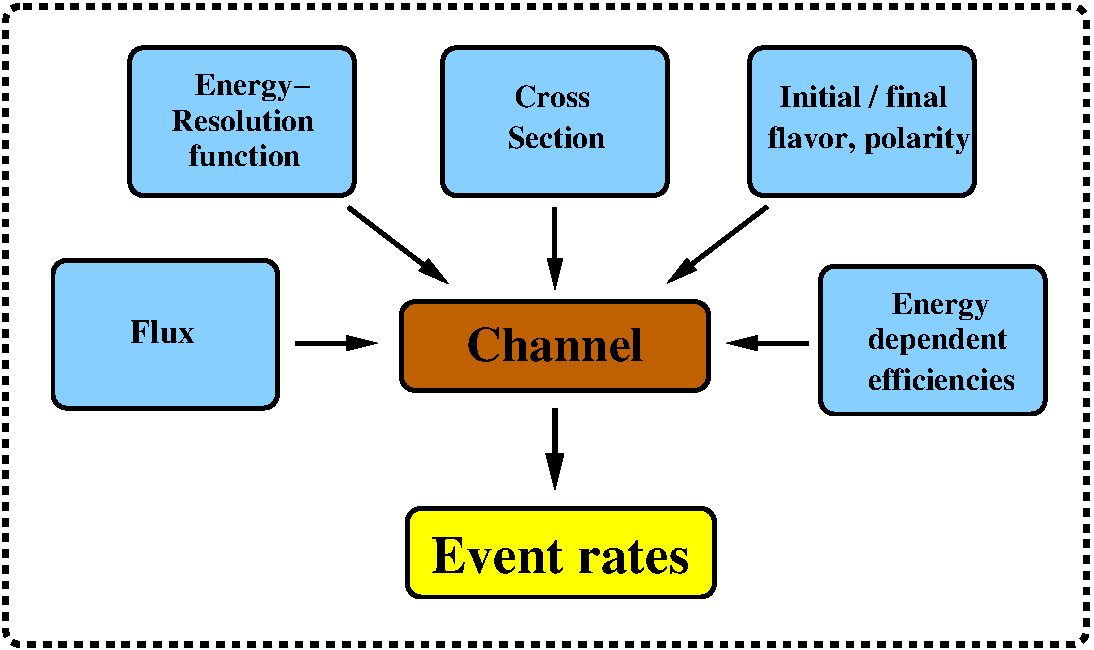
\includegraphics[width=19cm]{AEDL1}
    \end{center}
    A \emph{rule} consists of the combination of all signal and background
    channels in an experimental data sample (e.g.~$\nu_e$ appearance
    from $\nu_\mu \rightarrow \nu_e$ oscillations in a superbeam, with
    contamination from $\nu_e \rightarrow \nu_e$).

    \vspace{0.5cm}
    \begin{minipage}[T]{12cm}
      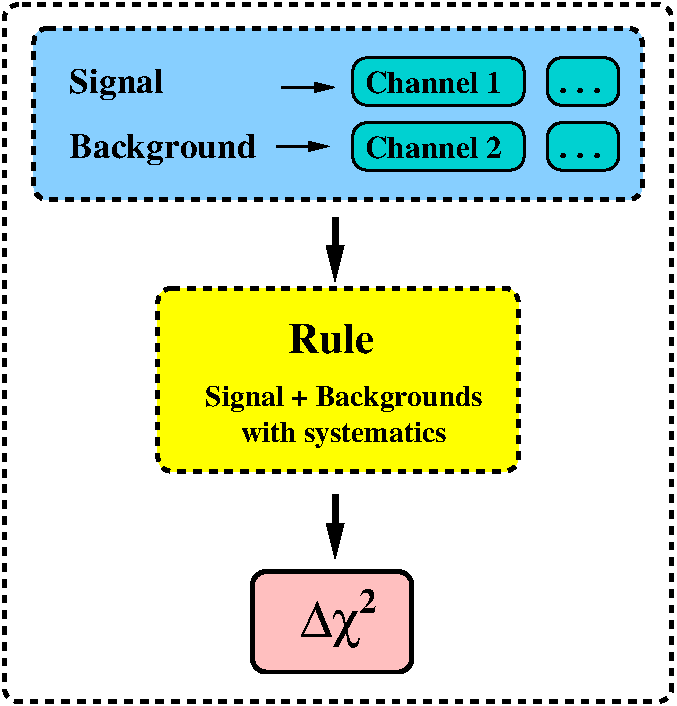
\includegraphics[width=12.5cm]{SignalBackground}
    \end{minipage}
    \hfill
    \begin{minipage}[T]{11.5cm}
      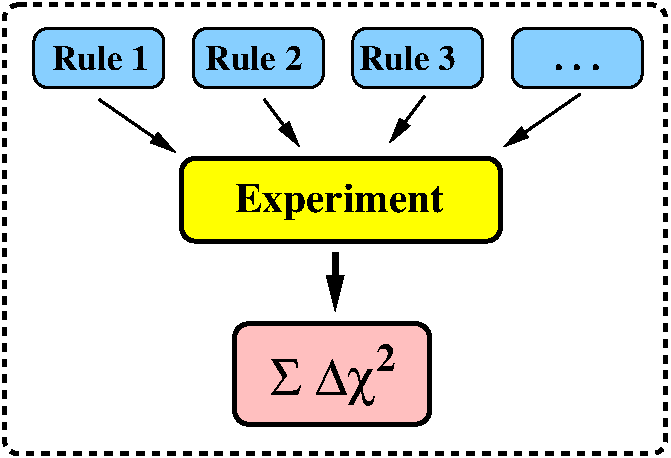
\includegraphics[width=11.5cm]{Rules}

      \vspace{-5.3cm}
      \cutout{r}(11.5cm,-7cm) \shapepar[27cm]{\circleshape}

      \emph{Experiments} can contain several rules, and several experiments
      can be handled simultaneously.
    \end{minipage}
    \hspace{0.5cm}
  }
  \hfill
  %
  \mytitlebox{18cm}{42cm}{Oscillations}{
    The oscillation engine is the heart of the software. Its main features
    are
    \begin{itemize}
      \item \emph{Full three-flavour treatment}
      \item \emph{Arbitrary (non-adiabatic) matter profiles} \\
        The PREM (Preliminary Reference Earth Model) matter profile
        is hard-coded in GLoBES. The user can choose approximations
        to this profile (e.g.~constant density, mantle-core-mantle
        profile, etc.)~or define completely new profiles.
      \item \emph{High numerical efficiency} \\
        GLoBES uses specifically designed numerical algorithms to
        ensure an excellent performance, which is, for the specific
        problem of neutrino oscillations, far superior to that of
        ``black box'' libraries.
      \item \emph{Extensibility} \\
        The user has the possibility to modify or completely replace
        the GLoBES oscillation engine, e.g.~to include sterile neutrinos,
        non-standard interactions, and other kinds of ``new physics''.
    \end{itemize}
  }
  \hfill
  %
  \mytitlebox{27cm}{42cm}{$\chi^2$ analysis}{
    GLoBES uses the \emph{$\chi^2$ method} to extract physical information
    from the simulated event spectra. Main features are
    \begin{itemize}
      \item \emph{Cuts and projections} of the multi-dimensional
        $\chi^2$ manifold (``marginalization'')
      \item Inclusion of \emph{systematical uncertainties}
        (fully customizable)
      \item Inclusion of \emph{correlations and degeneracies}
      \item Inclusion of \emph{external priors}
        (fully customizable)
      \item Supports setups with \emph{Multiple sources} and
        \emph{multiple detectors}
      \item Excellent \emph{numerical efficiency}
    \end{itemize}
    The builtin $\chi^2$ functions of GLoBES have the Poissonian form
    \begin{align*}
      \chi^2(\vec{\lambda}, \vec{a})
        =& 2 \sum_{\rm exp's} \sum_{\rm rules} \sum_{\rm bins}
          \Bigg[
              N^{\rm th}(\vec{\lambda}, \vec{a}) - N^{\rm obs}
            + N^{\rm obs} \log\frac{N^{\rm obs}}{N^{\rm th}(\vec{\lambda}, \vec{a})}
          \Bigg] \\[0.5cm]
         & + \chi^2_{\rm prior}(\vec{\lambda}) + \chi^2_{\rm pull}(\vec{a}),
    \end{align*}
    where $N^{\rm obs}$ and $N^{\rm th}$ are the ``observed'' and
    theoretically predicted event rates, respectively. The vector $\vec{\lambda}$
    contains the oscillation parameters, and $\vec{a}$ are the systematical biases.
    $\chi^2_{\rm prior}(\vec{\lambda})$ and $\chi^2_{\rm pull}(\vec{a})$
    implement external input on these parameters. Note that GLoBES allows
    also for \emph{arbitrary, user-defined $\chi^2$ functions}.

    \vspace{0.5cm}
    \emph{\bf Example:}
    $\theta_{13}$--$\delta_{\rm CP}$ correlation and intrinsic degeneracy
    in a $\nu$-fact.

    \hspace*{0.5cm} 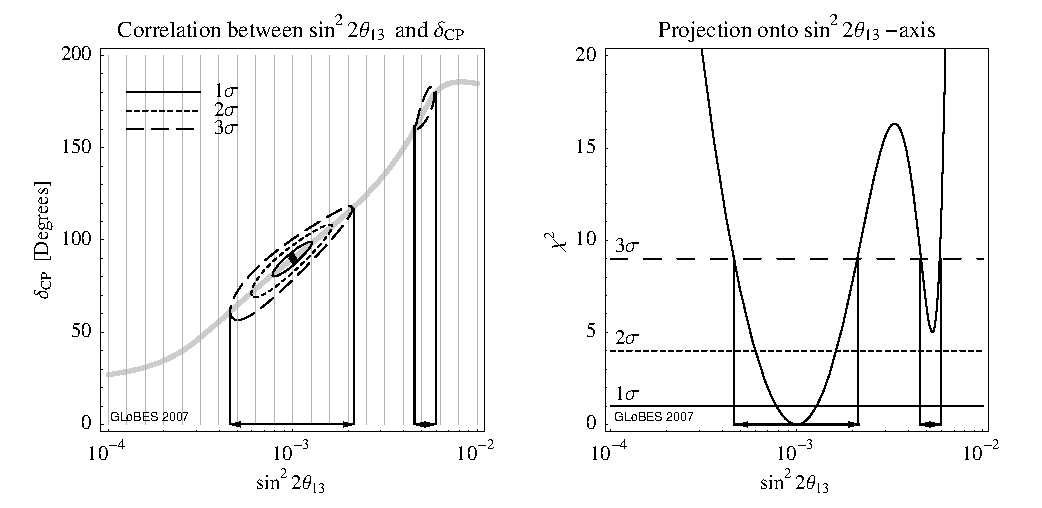
\includegraphics[width=25.5cm]{projex}
    \vspace{-1cm}
  }
  \hspace*{1cm}
\end{center}
%
\vspace{1.0cm}
%
%--------------------------------------------------------------
% Second row of boxes
%--------------------------------------------------------------
\begin{center}
  \hspace*{1cm}
  \mytitlebox{24cm}{36cm}{GLoBES example}{
  \emph{\bf The AEDL file:} A simple neutrino factory

    \vspace{\topsep}
    \begin{tikzpicture}%
      \draw [fill=white,rounded corners=0pt]%
        (0cm,0cm) node [anchor=north west] at (0cm,-0.2cm){%
          \begin{minipage}[t]{9cm}
            \tt\footnotesize
            \hspace*{0.0cm} \$version=\dr{"3.0.0"}                       \\
            \hspace*{0.0cm} nuflux(\dg{\#mu\_plus})<                     \\
            \hspace*{0.5cm}   @builtin = \dr{1}                          \\
            \hspace*{0.5cm}   @parent\_energy = \dr{50}                  \\
            \hspace*{0.5cm}   @stored\_muons = \dr{10.66e+20}            \\
            \hspace*{0.5cm}   @time = \dr{4}                             \\
            \hspace*{0.0cm} >                                            \\
            \hspace*{0.0cm} \$target\_mass = \dr{50}                     \\
            \hspace*{0.0cm} \$bins = \dr{20}                             \\
            \hspace*{0.0cm} \$emin = \dr{ 4}                             \\
            \hspace*{0.0cm} \$emax = \dr{50}                             \\
            \hspace*{0.0cm} \$profiletype = \dr{1}                       \\
            \hspace*{0.0cm} \$baseline = \dr{3000}                       \\
            \hspace*{0.0cm} energy(\dg{\#ERES})< \db{/*E res.*/}         \\
            \hspace*{0.5cm}   @type = \dr{1}                             \\
            \hspace*{0.5cm}   @sigma\_e = \{\dr{0.15}, \dr{0}, \dr{0}\}  \\
            \hspace*{0.0cm} >
          \end{minipage}
          %
          \hfill
          %
          \begin{minipage}[t]{16cm}
            \tt\footnotesize
            \hspace*{0.0cm} cross(\dg{\#CC})<   \db{/* Cross sections */}\\
            \hspace*{0.5cm}   @cross\_file = \dr{"XCC.dat"}              \\
            \hspace*{0.0cm} >                                            \\
            \hspace*{0.0cm} channel(\dg{\#nu\_mu\_app})<                 \\
            \hspace*{0.5cm}   @channel = \dg{\#mu\_plus}:\dr{+}:\dr{e}:\dr{m}:\dg{\#CC}:\dg{\#ERES} \\
            \hspace*{0.0cm} >                                            \\
            \hspace*{0.0cm} channel(\dg{\#nu\_mu\_bar\_disapp})<         \\
            \hspace*{0.5cm}   @channel = \dg{\#mu\_plus}:\dr{-}:\dr{m}:\dr{m}:\dg{\#CC}:\dg{\#ERES} \\
            \hspace*{0.0cm} >                                            \\
            \hspace*{0.0cm} rule(\dg{\#Nu\_Mu\_Appearance})<             \\
            \hspace*{0.5cm}   @signal = \dr{0.45}@\dg{\#nu\_mu\_app}     \\
            \hspace*{0.5cm}   @signalerror = \dr{0.025} : \dr{0.0001}    \\
            \hspace*{0.5cm}   @background  = \dr{5e-6}@\dg{\#nu\_mu\_bar\_disapp} \\
            \hspace*{0.5cm}   @backgrounderror = \dr{0.2} : \dr{0.0001}  \\
            \hspace*{0.5cm}   @sys\_on\_function = \dr{"chiSpectrumTilt"}\\
            \hspace*{0.5cm}   @sys\_off\_function = \dr{"chiNoSysSpectrum"} \\
            \hspace*{0.0cm} >
          \end{minipage}}%
        rectangle (22.5cm,-14cm);
      \draw (9.5cm,-0.5cm) -- (9.5cm,-13.5cm);
    \end{tikzpicture}%

    \vspace{0.5cm}
    \emph{\bf Application code snippet:} Project $\chi^2$ onto $\theta_{13}$ axis

    \vspace{\topsep}
    \begin{tikzpicture}%
      \draw [fill=white,rounded corners=0pt]%
        (0cm,0cm) node [anchor=north west] at (0cm,-0.2cm){%
          \begin{minipage}[t]{25cm}
            \tt\footnotesize
            \hspace*{0.0cm} \db{/* Define priors for $\theta_{12}$ and $\Delta m_{21}^2$ */} \\
            \hspace*{0.0cm} glbDefineParams(input\_errors, theta12*\dr{0.1}, \dr{0},
                              \dr{0}, \dr{0}, sdm*\dr{0.1}, \dr{0}); \\
            \hspace*{0.0cm} glbSetDensityParams(input\_errors, \dr{0.05}, GLB\_ALL);    \\
            \hspace*{0.0cm} glbSetCentralValues(true\_values);                          \\
            \hspace*{0.0cm} glbSetInputErrors(input\_errors);                           \\
            \hspace*{0.0cm}                                                             \\
            \hspace*{0.0cm} \db{/* Loop over $\log(\sin^2 2\theta_{13})$ */}            \\
            \hspace*{0.0cm} \dg{double} theta13, x;                                     \\
            \hspace*{0.0cm} \dy{for} (x=\dr{-4}; x < \dr{-2.0}+\dr{0.001}; x+=\dr{2.0}/\dr{50})\\
            \hspace*{0.0cm} \{                                                          \\
            \hspace*{0.5cm}   theta13 = asin(sqrt(pow(\dr{10},x)))/\dr{2};              \\
            \hspace*{0.5cm}                                                             \\
            \hspace*{0.5cm}   \db{/* Choose starting value for $\delta_{CP}$ marginalization */} \\
            \hspace*{0.5cm}   glbSetOscParams(test\_values,
                               \dr{200.0}/\dr{2}*(x+\dr{4})*\dr{M\_PI}/\dr{180}, GLB\_DELTA\_CP); \\
            \hspace*{0.5cm}                                                             \\
            \hspace*{0.5cm}   \db{/* Compute $\chi^2$ and marginalize over all parameters
                                                                except $\theta_{13}$ */}\\
            \hspace*{0.5cm}   chi2 = glbChiTheta13(test\_values, \dr{NULL}, GLB\_ALL);  \\
            \hspace*{0.0cm} \}
          \end{minipage}}%
        rectangle (22.5cm,-15cm);
    \end{tikzpicture}%
  }
  \hfill
  %
  \mybox{24cm}{36cm}{
    \vspace{12cm}
    \large
    {\bf GLoBES website:}
    \begin{center}
      {\tt\emph{www.mpi-hd.mpg.de/$\sim$globes/}}
    \end{center}

    \vspace{0.5cm}
    \hspace*{0.5cm}
    \begin{minipage}{15cm}
      \begin{itemize}
        \item Software download
        \item Many predefined AEDL files
        \item Extensive documentation
        \item Examples and tutorials
      \end{itemize}
    \end{minipage}

    \vspace{1cm}
    {\bf GLoBES publications:}
    \begin{center}
      CPC {\bf 167}, 195 (2005), {\tt hep-ph/0407333} \\
      CPC {\bf 177}, 432 (2007), {\tt hep-ph/0701187}
    \end{center}

    \vspace{0.5cm}
    {\bf Contact the authors:}
    \begin{center}
      {\tt\emph{globes@mpi-hd.mpg.de}}
    \end{center}

    \vspace{1.0cm}
    \begin{center}
      
\includegraphics[height=3cm]{cern-logo}      \hspace{0.5cm}
      
\includegraphics[height=3cm]{vt-logo}        \hspace{0.5cm}
      
\includegraphics[height=3cm]{minerva}        \hspace{0.5cm}
      
\includegraphics[height=3cm]{wuerzburg-logo} \hspace{0.5cm}
    \end{center}
  }
  \hfill
  %
  \mytitlebox{24cm}{36cm}{Recent GLoBES results}{
    \small
    \vspace{1.0cm}
    \hspace{-0.7cm}
    \begin{tabular}{c|c}
      \begin{minipage}[t]{11cm}
        \vspace{0.2cm}
        \emph{\bf Evolution of $\sin^2 2\theta_{13}$ disc.~reach} \\[0.5cm]
        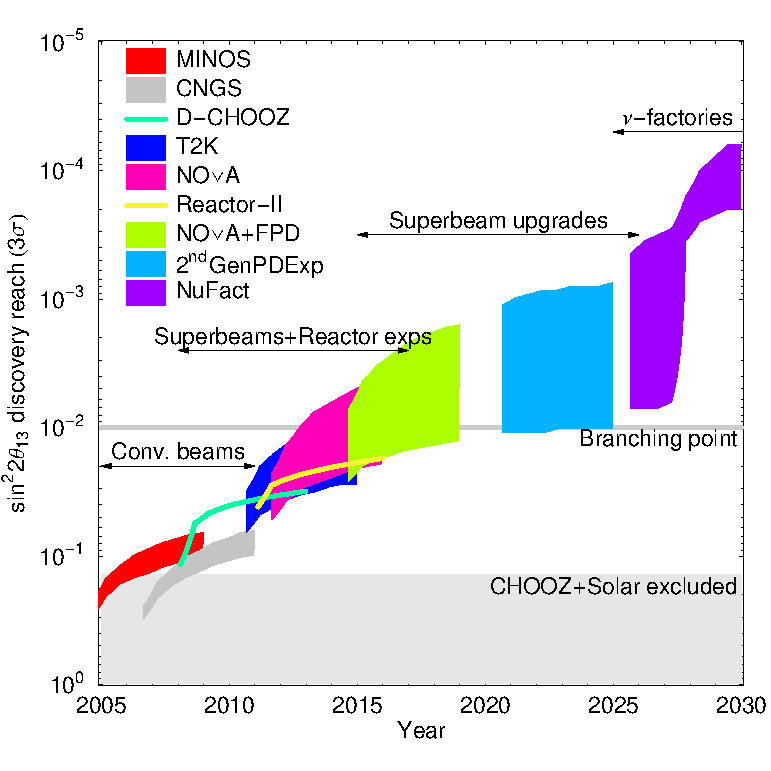
\includegraphics[width=11cm]{disclimitbandnova}
      \end{minipage}
      %
      &
      %
      \begin{minipage}[t]{12cm}
        \vspace{0.2cm}
        \emph{\bf $\delta_{CP}$ sensitivity of different exp's} \\[0.5cm]
        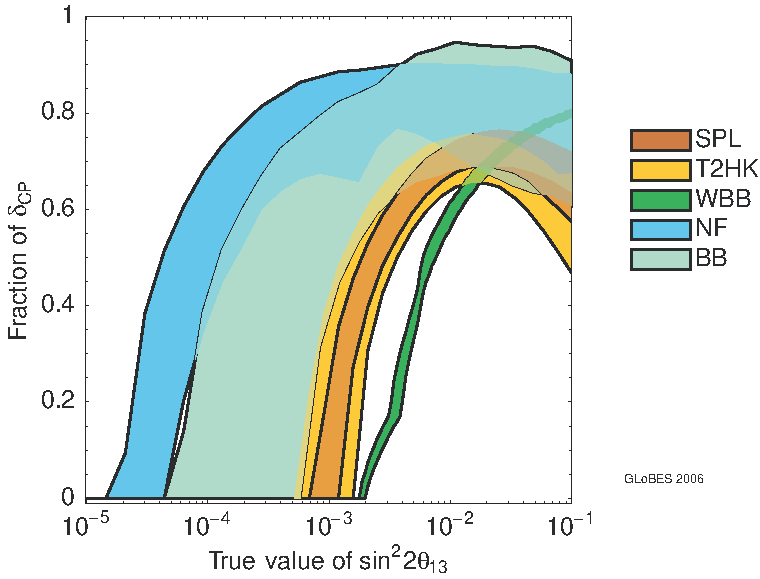
\includegraphics[width=12cm]{cpv-1}
      \end{minipage}
      %
      \\ %\hline
      %
      \begin{minipage}[t]{11cm}
        \raggedright
        \vspace{0.5cm}
        \emph{\bf Impact of systematical errors in a reactor experiment} \\[0.5cm]
        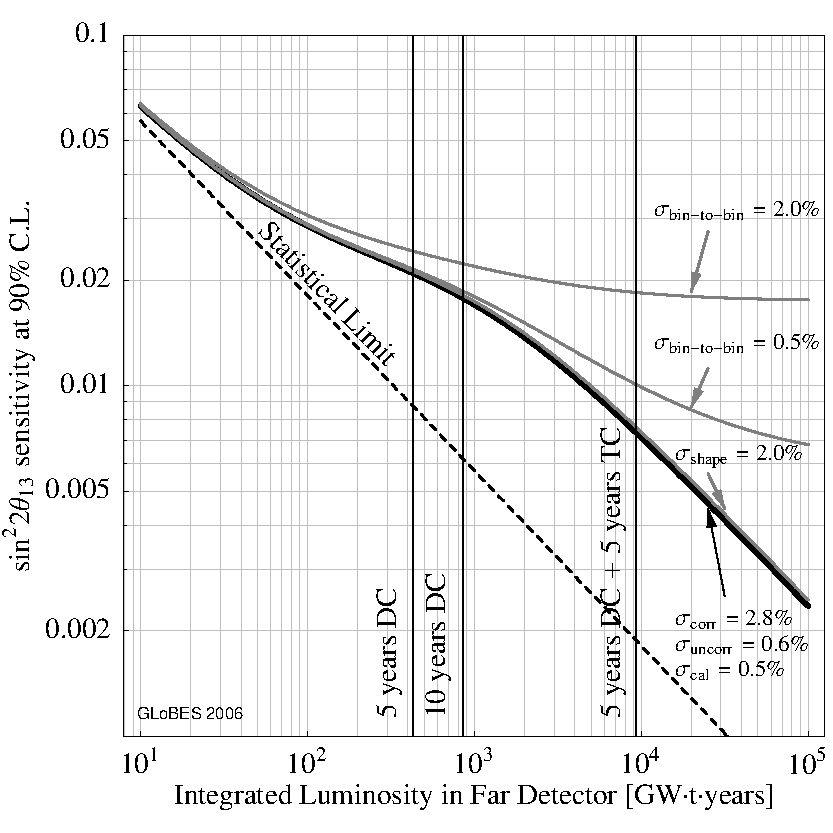
\includegraphics[width=11cm]{systematics}
      \end{minipage}
      %
      &
      %
      \begin{minipage}[t]{12cm}
        \vspace{-1.5cm}
        \emph{\bf Sensitivity of $\nu$-fact to standard and non-standard physics} \\[0.5cm]
        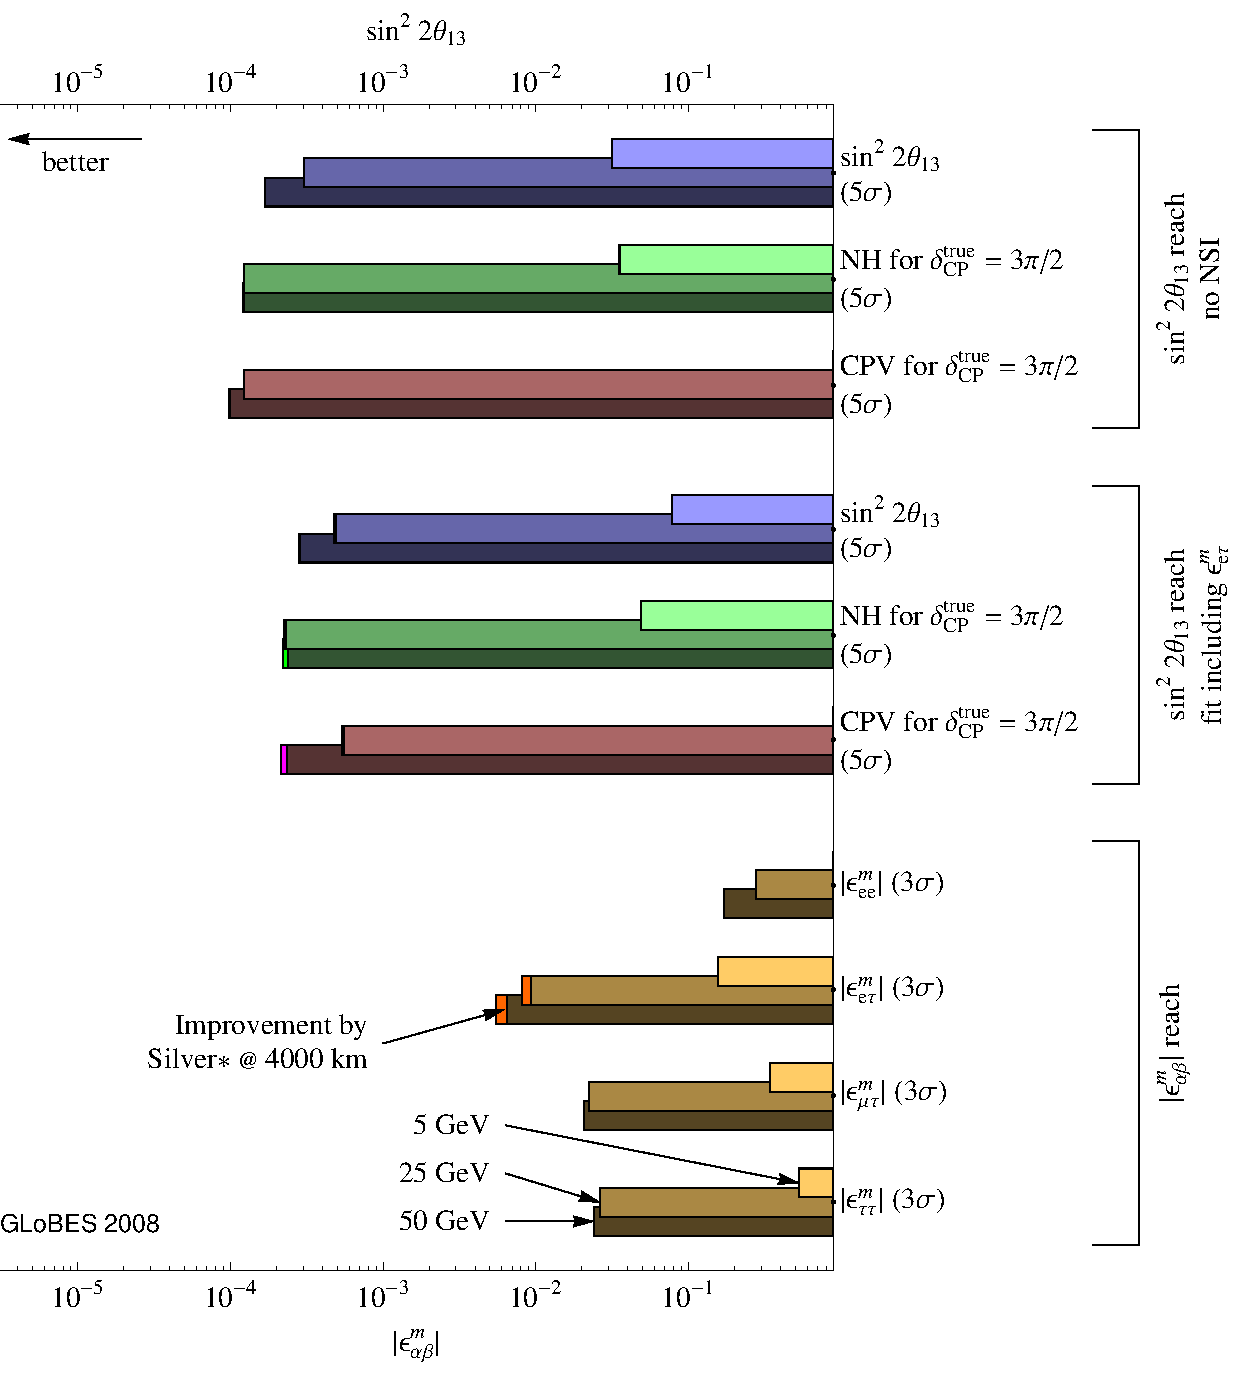
\includegraphics[width=12cm]{bar-chart}
      \end{minipage}
    \end{tabular}
  }
  \hspace*{1cm}
\end{center}
\vspace{1cm}
%
%--------------------------------------------------------------
% GLoBES Logo
%--------------------------------------------------------------
\begin{tikzpicture}[remember picture,overlay]
    \fill[fill=bgcolor] (38.85cm, 40.5cm) circle (13.5cm);
    \node[inner sep=0pt] at (38.85cm, 40.5cm) {
      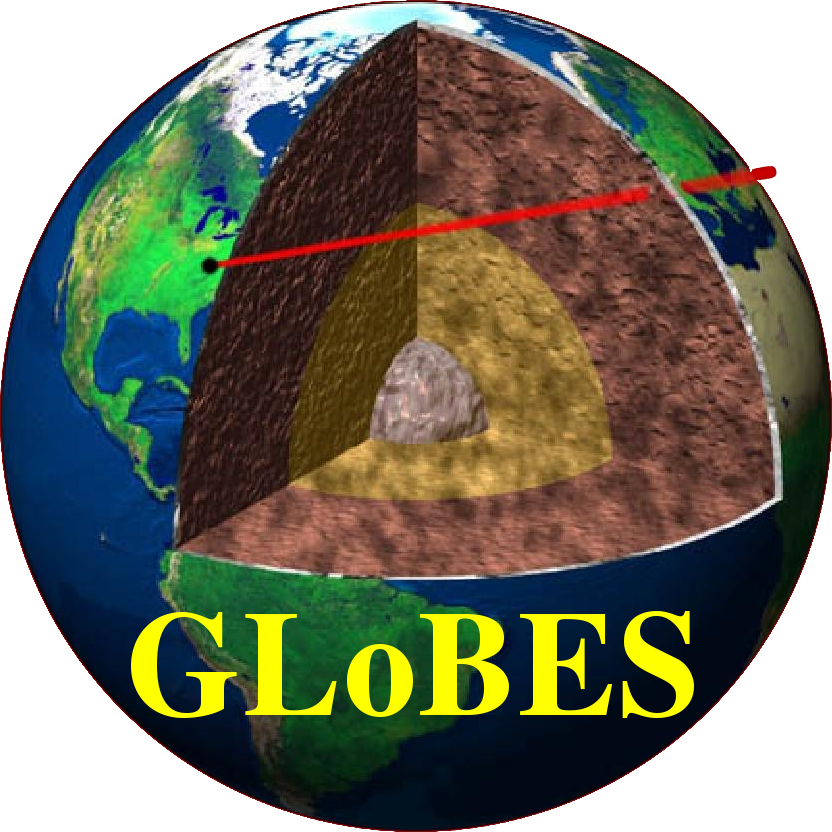
\includegraphics[width=22cm,height=22cm]{globes-red.png}
    };
\end{tikzpicture}


%--------------------------------------------------------------
% Background II
%--------------------------------------------------------------
\end{minipage}}

\end{document}





